%!TEX root = Report.tex

\section{Introduction}

% Many species of termites, including ants, work in swarms to build structures that are many times larger than themselves. The fact that they do this in an efficient manner makes termites an interesting subject for study because we, as humans, can hope to learn from their techniques and apply them in a human context in construction of houses, bridges etc. Studying termite behavior, however, requires a lab environment facilitating appropriate hard- and software tools. \\
% 
% The goal of the Self-Organizing Systems Research Group (SOSRG) at Harvard University is to develop a swarm construction system in which robots cooperate to build 3D structures much larger than themselves. As of this writing, the system consists of simple robots that are able to move around and cooperate in and combining physical objects in order to build larger user defined pieces from high level descriptions. \\
% 
% This project is conducted at the IT University of Copenhagen (ITU) in the fall 2013 in cooperation with SOSRG. The goal of the project is to build software to interface with Harvard hardware in order to create a stand-alone environment for tracking and monitoring termites. Specifically, \\

This report is written at the IT University of Copenhagen (ITU) in the fall term of 2013 as a project supervised by Kasper Støy from ITU and with additional guidance from Kirstin Petersen from Harvard University. The project was developed from September 1st to December 16th 2013. The report is addressed to people interested in tracking ants or termites using image analysis. \\

%• General statement introducing the area; \\
%You can most likely start with the first paragraph from your project description and evolve it. - 
The Self-Organizing Systems Research Lab at Harvard University has created an autonomous robot for tracking African termites in a lab environment but lacks the necessary software support. Working with and tracking these termites is cumbersome as they only thrive in environments that resemble their native environment and only when they are together with other termites. Therefore automatic tracking of specific termites is necessary, as tracking up until now has been done manually. \\

%• Explanation of the specific problem and why do we care about the problem. (MOTIVATON)\\
This project aims to develop software that is able to track both ants and termites in their native environment using a Hewlett-Packard XY-plotter provided by Harvard University. While it is already possible to communicate with the plotter using for instance Termite \cite{termite}, there is a need for software that integrates tracking, plotter communication, statistics and a graphical user interface. The end product is to be used by biologists and this software will lay the foundation to enable them to track ants/termites with more precision and with better data being collected. Since biologists who are the future end users of the product would like to be able to stimulate the ants/termites with food and/or pheromon, we need a non-stationary part which is exactly what the plotter provides (the XY-arm) \\

%• Explanation of your solution, and how it improves on the work by others. Relation to related work can be very brief, given that you have a separate extensive section devoted to this. \\
A team at Harvard University previously experimented \todo{kan vi få en ref til deres projekt?}with using the plotter to track a single ant/termite on a white background with some success. While the details of this effort were unknown to us we decided to start this project from scracth. Since this team had some success with their approach we use their hardware setup as a starting point for this project. The focus of the project is mainly on the development of the software and the selected hardware has a secondary role. \\



\begin{figure}
        \centering
        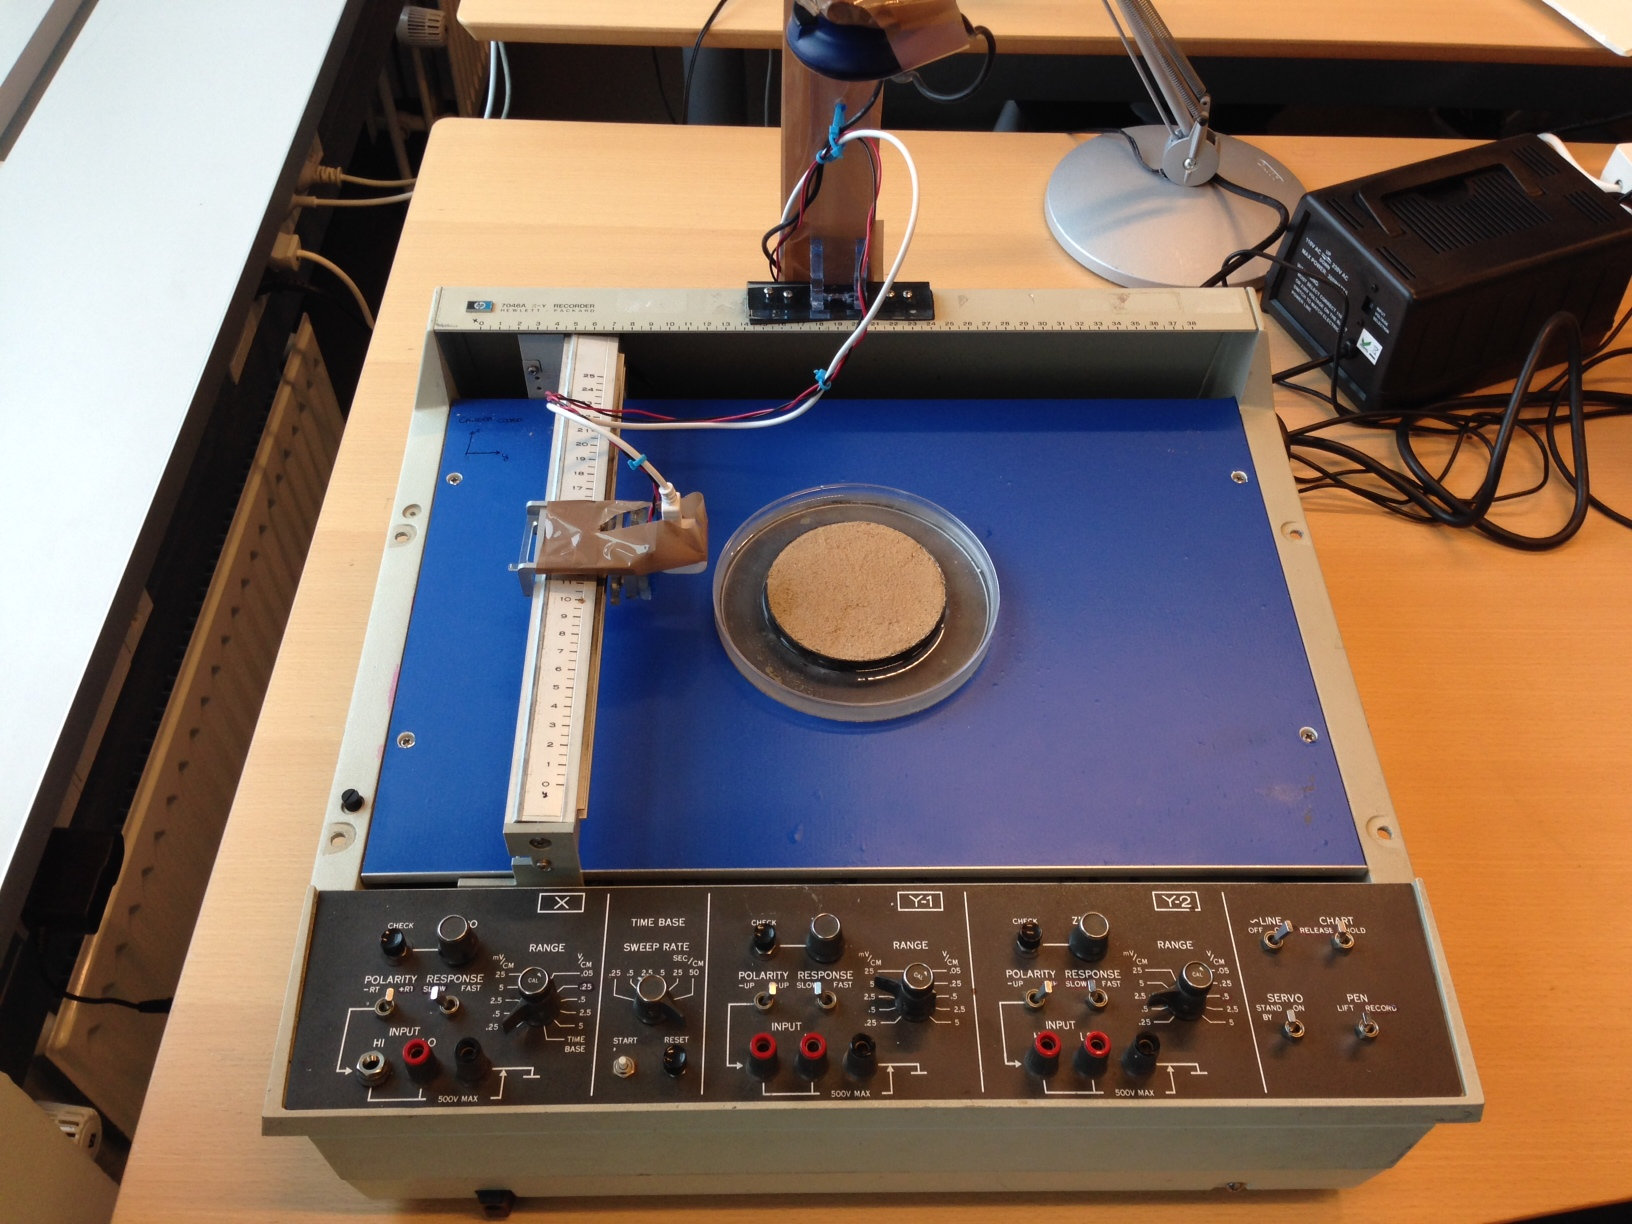
\includegraphics[scale=0.125]{img/plotter}
        \caption{Plotter with mobile camera, overhead camera and control panel}
        \label{fig:plotter}
\end{figure}

%• A hint on how the solution was evaluated and what was the outcome of this evaluation. \\
Since tracking of ants/termites is very hard to test systematically we have chosen to evaluate it by describing in what instances we expect the tracking to work as intended and in what instances we expect it not to. The results show that the tracking of the ants/termites are both possible and satisfactory but still have situations where the it will fail. Both the results and possible solutions improvements can be found in section \ref{testing} Testing the tracking software with real ants \\

This project was undertaken as a substitute for the "Global Software Development" course at ITU and therefore has additional emphasis on the international collaboration and developement process. Section \ref{process} Process will describe the tools used as well as evaluate the overall process. \\ 

%A summary (a “map”) of how the paper is organized.\\
This report assumes that the reader has a basic knowledge of mathematics but any prior knowledge about computer vision is not required. We will first describe the requirements and scope of the project and the tracking theory we either considered or used in the project. Then we will describe how we interacted with the XY-plotter and how we built the tracking and interaction together. Lastly will we describe the tests, analyze the results and conclude the project.



